\usetikzlibrary{fit, calc, positioning, arrows.meta}
\usetikzlibrary{shapes.multipart, positioning, arrows.meta, calc}

\chapter{Rappresentazione di insiemi disgiunti mediante Liste Concatenate}
\section{Struttura della lista}
\begin{itemize}
    \item Ogni insieme è rappresentato mediante una lista
    \item Oggeto di un insieme (uno per ciascun insieme)
    \begin{itemize}
        \item \textbf{Head:} punta al 1° oggetto in lista
        \item \textbf{Tail:} punta all'ultimo oggetto in lista
    \end{itemize}

    \begin{figure}[htbp]
    \centering
        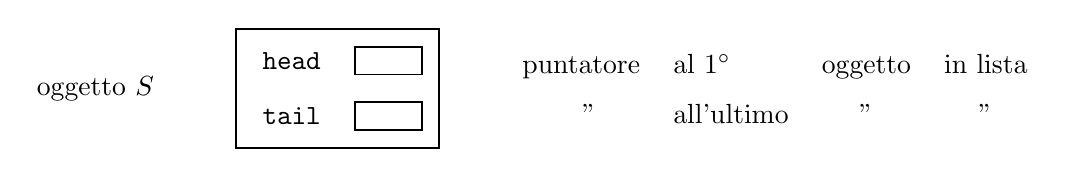
\begin{tikzpicture}[
            slot/.style={draw=black, semithick, minimum width=0.85cm, minimum height=0.35cm, inner sep=0pt},
            every node/.style={font=\normalsize}
        ]
            % Etichetta a sinistra
            \node (s_label) at (0, 0) {oggetto $S$};

            % Campi interni (head e tail)
            \node[anchor=west] (head_lbl) at (2.0, 0.35) {\texttt{head}};
            \node[slot, right=3mm of head_lbl] (head_ptr) {};

            \node[anchor=west] (tail_lbl) at (2.0, -0.35) {\texttt{tail}};
            \node[slot, right=3mm of tail_lbl] (tail_ptr) {};

            % Riquadro esterno dell'oggetto S
            \node[draw=black, thick, fit=(head_lbl) (head_ptr) (tail_lbl) (tail_ptr), inner xsep=6pt, inner ysep=5pt] (boxS) {};

            % Annotazioni a destra con incolonnamento delle virgolette
            \node[anchor=west, right=8mm of boxS.east] (desc) {
                \renewcommand{\arraystretch}{1.5}
                \begin{tabular}{@{}l l c c@{}}
                    puntatore & al $1^\circ$ & oggetto & in lista \\
                    \multicolumn{1}{c}{''} & all'ultimo & '' & ''
                \end{tabular}
            };
        \end{tikzpicture}
    \end{figure}

    \item Oggetto di una lista
    \begin{itemize}
        \item \textbf{set:} Puntatore all'oggetto dell'insieme
        \item \textbf{key:} Elemento dell'insieme
        \item \textbf{next:} Puntatore all'oggetto della lista dove contiene un altro elemento dell'insieme (oppure NIL)
    \end{itemize}

    \begin{figure}[htbp]
    \centering
    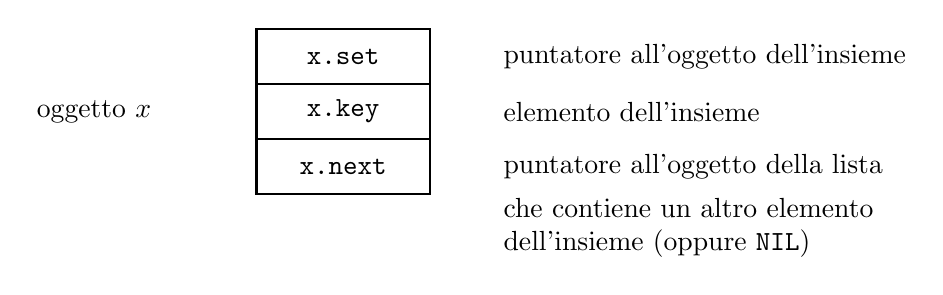
\begin{tikzpicture}[
        cell/.style={draw=black, thick, minimum width=2.2cm, minimum height=0.7cm, font=\ttfamily},
        every node/.style={font=\normalsize}
    ]
        % Riquadro dell'oggetto x (tre campi impilati)
        \node[cell] (set) {x.set};
        \node[cell, below=-\pgflinewidth of set] (key) {x.key};
        \node[cell, below=-\pgflinewidth of key] (next) {x.next};

        % Etichetta a sinistra (allineata al campo centrale)
        \node[left=1.2cm of key] (x_label) {oggetto $x$};

        % Annotazioni a destra
        \node[anchor=west, right=8mm of set] (desc_set) {puntatore all'oggetto dell'insieme};
        \node[anchor=west, right=8mm of key] (desc_key) {elemento dell'insieme};
        \node[anchor=west, right=8mm of next] (desc_next) {puntatore all'oggetto della lista};

        % Righe a capo per la descrizione di x.next perfettamente allineate
        \node[anchor=north west, align=left] at (desc_next.south west) {
            che contiene un altro elemento \\
            dell'insieme (oppure \texttt{NIL})
        };
    \end{tikzpicture}
    \end{figure}

    \item Il rappresentante è il 1° oggetto della lista
    

\end{itemize}

\begin{figure}[htbp]
\centering
% Definizione dell'insieme in alto
\noindent \underline{\textbf{ES:}} \quad $S^2 = \{c, h, e, b\}$

\vspace{0.8cm}

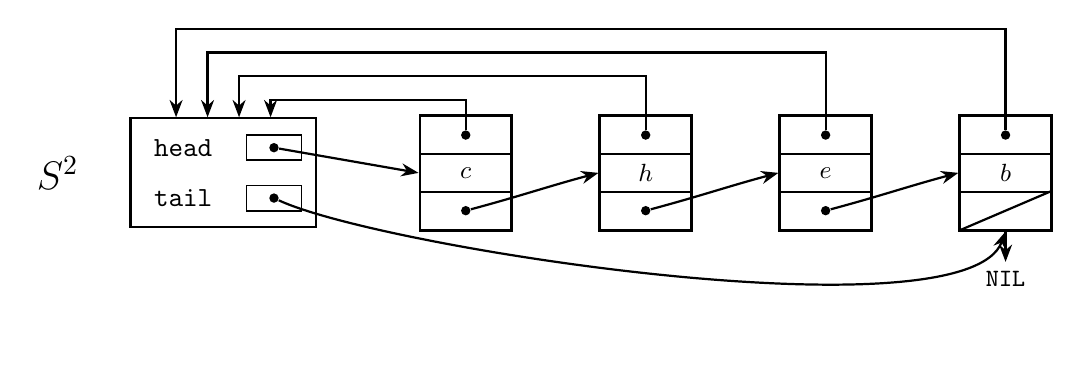
\begin{tikzpicture}[
    slot/.style={draw=black, semithick, minimum width=0.7cm, minimum height=0.32cm, inner sep=0pt},
    cell/.style={draw=black, semithick, minimum width=1.15cm, minimum height=0.48cm, font=\small},
    arr/.style={-{Stealth[length=2.2mm]}, thick},
    ptr/.style={circle, fill=black, inner sep=1.2pt}
]
    % --- 1. Riquadro Oggetto Insieme S^2 (a sinistra) ---
    \node[font=\bfseries\Large] (s2_lbl) at (-1.1, 0) {$S^2$};

    \node[anchor=west] (head_lbl) at (0, 0.32) {\texttt{head}};
    \node[slot, right=3mm of head_lbl] (head_slot) {};

    \node[anchor=west] (tail_lbl) at (0, -0.32) {\texttt{tail}};
    \node[slot, right=3mm of tail_lbl] (tail_slot) {};

    \node[draw=black, thick, fit=(head_lbl) (head_slot) (tail_lbl) (tail_slot), inner xsep=5pt, inner ysep=4pt] (boxS2) {};

    % --- 2. Elementi della lista concatenata (c, h, e, b) ---
    % Nodo 'c' (rappresentante)
    \node[cell, right=1.3cm of boxS2] (c_key) {$c$};
    \node[cell, above=-\pgflinewidth of c_key] (c_set) {};
    \node[cell, below=-\pgflinewidth of c_key] (c_next) {};
    \node[draw=black, thick, fit=(c_set) (c_next), inner sep=0pt] (box_c) {};

    % Nodo 'h'
    \node[cell, right=1.1cm of box_c.east |- c_key] (h_key) {$h$};
    \node[cell, above=-\pgflinewidth of h_key] (h_set) {};
    \node[cell, below=-\pgflinewidth of h_key] (h_next) {};
    \node[draw=black, thick, fit=(h_set) (h_next), inner sep=0pt] (box_h) {};

    % Nodo 'e'
    \node[cell, right=1.1cm of box_h.east |- h_key] (e_key) {$e$};
    \node[cell, above=-\pgflinewidth of e_key] (e_set) {};
    \node[cell, below=-\pgflinewidth of e_key] (e_next) {};
    \node[draw=black, thick, fit=(e_set) (e_next), inner sep=0pt] (box_e) {};

    % Nodo 'b' (ultimo elemento)
    \node[cell, right=1.1cm of box_e.east |- e_key] (b_key) {$b$};
    \node[cell, above=-\pgflinewidth of b_key] (b_set) {};
    \node[cell, below=-\pgflinewidth of b_key] (b_next) {};
    \node[draw=black, thick, fit=(b_set) (b_next), inner sep=0pt] (box_b) {};

    % --- 3. Punti di origine dei puntatori ---
    \node[ptr] (pt_head) at (head_slot.center) {};
    \node[ptr] (pt_tail) at (tail_slot.center) {};
    \node[ptr] (pt_c_set) at (c_set.center) {};
    \node[ptr] (pt_h_set) at (h_set.center) {};
    \node[ptr] (pt_e_set) at (e_set.center) {};
    \node[ptr] (pt_b_set) at (b_set.center) {};
    \node[ptr] (pt_c_next) at (c_next.center) {};
    \node[ptr] (pt_h_next) at (h_next.center) {};
    \node[ptr] (pt_e_next) at (e_next.center) {};

    % --- 4. Collegamenti head e next ---
    \draw[arr] (pt_head) -- (box_c.west |- c_key);
    \draw[arr] (pt_c_next) to[out=15, in=195] (box_h.west |- h_key);
    \draw[arr] (pt_h_next) to[out=15, in=195] (box_e.west |- e_key);
    \draw[arr] (pt_e_next) to[out=15, in=195] (box_b.west |- b_key);

    % Terminazione NIL per il nodo 'b'
    \draw[thick] (b_next.south west) -- (b_next.north east);
\node[below=4mm of b_next, font=\small\ttfamily] (nil) {NIL};    \draw[arr] (b_next.south) -- (nil.north);

    % --- 5. Puntatore tail (curva sotto tutti i blocchi) ---
    \draw[arr] (pt_tail) to[out=-25, in=-110, looseness=0.4] (box_b.south);

    % --- 6. Puntatori x.set (archi superiori verso S^2) ---
    \draw[arr] (pt_c_set) -- ++(0, 0.45) -| ([xshift=6mm]boxS2.north);
    \draw[arr] (pt_h_set) -- ++(0, 0.75) -| ([xshift=2mm]boxS2.north);
    \draw[arr] (pt_e_set) -- ++(0, 1.05) -| ([xshift=-2mm]boxS2.north);
    \draw[arr] (pt_b_set) -- ++(0, 1.35) -| ([xshift=-6mm]boxS2.north);

\end{tikzpicture}
\caption*{Rappresentazione con lista concatenata dell'insieme $S^2 = \{c, h, e, b\}$.}
\end{figure}

\newpage
\section{Metodi della lista}

\subsection{Make-Set}
Dato l'oggetto x si vuole creare una lista S avente x come unico oggetto

\begin{minipage}{0.45\textwidth}
    \begin{figure}[H]
        \centering
        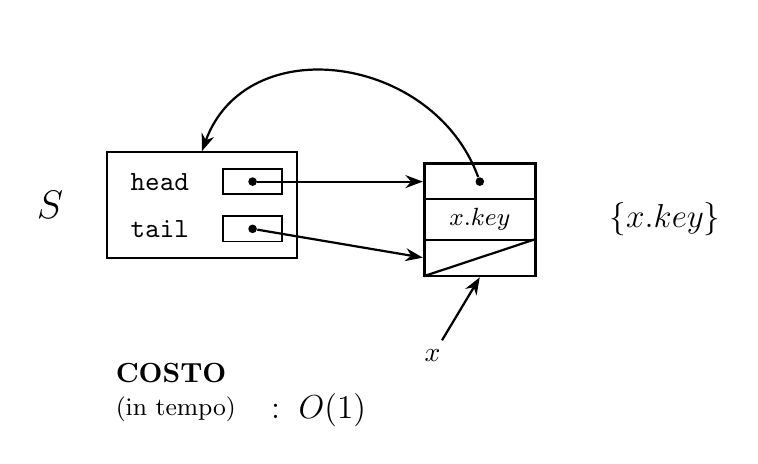
\begin{tikzpicture}[
            slot/.style={draw=black, semithick, minimum width=0.75cm, minimum height=0.32cm, inner sep=0pt},
            cell/.style={draw=black, semithick, minimum width=1.4cm, minimum height=0.45cm, font=\small},
            arr/.style={-{Stealth[length=2.2mm]}, thick},
            ptr/.style={circle, fill=black, inner sep=1.1pt}
        ]
            % --- Oggetto Insieme S (a sinistra) ---
            \node[font=\bfseries\Large] (s_lbl) at (-0.9, 0) {$S$};

            \node[anchor=west] (head_lbl) at (0, 0.3) {\texttt{head}};
            \node[slot, right=3mm of head_lbl] (head_slot) {};

            \node[anchor=west] (tail_lbl) at (0, -0.3) {\texttt{tail}};
            \node[slot, right=3mm of tail_lbl] (tail_slot) {};

            \node[draw=black, thick, fit=(head_lbl) (head_slot) (tail_lbl) (tail_slot), inner xsep=5pt, inner ysep=4pt] (boxS) {};

            % --- Elemento x (a destra) ---
            \node[cell, right=1.6cm of boxS.east |- head_slot] (x_set) {};
            \node[cell, below=-\pgflinewidth of x_set] (x_key) {$x.key$};
            \node[cell, below=-\pgflinewidth of x_key] (x_next) {};
            \node[draw=black, thick, fit=(x_set) (x_next), inner sep=0pt] (box_x) {};

            % Tratto obliquo su next (rappresenta puntatore a NIL)
            \draw[thick] (x_next.south west) -- (x_next.north east);

            % Punti di origine dei puntatori
            \node[ptr] (pt_head) at (head_slot.center) {};
            \node[ptr] (pt_tail) at (tail_slot.center) {};
            \node[ptr] (pt_set) at (x_set.center) {};

            % Frecce da head e tail verso l'oggetto x
            \draw[arr] (pt_head) -- (box_x.west |- x_set);
            \draw[arr] (pt_tail) -- (box_x.west |- x_next);

            % Freccia x.set di ritorno verso l'oggetto insieme S
            \draw[arr] (pt_set) to[out=110, in=70, looseness=1.2] (boxS.north);

            % Puntatore della variabile x dal basso verso il blocco
            \node (x_var) at ([shift={(-0.6cm, -1.0cm)}]box_x.south) {$x$};
            \draw[arr] (x_var) -- (box_x.south);

            % Rappresentazione dell'insieme a destra
            \node[right=0.8cm of box_x.east, font=\large] (set_repr) {$\{x.key\}$};

            % Costo temporale in basso
            \node[anchor=north west, align=left, font=\normalsize] (cost) at ([yshift=-1.2cm]boxS.south west) {
                \textbf{COSTO} \\
                \small (in tempo)
            };
            \node[right=2mm of cost.mid east, font=\large] (cost_val) {$: \; O(1)$};

        \end{tikzpicture}
    \end{figure}
\end{minipage}
\hfill
\begin{minipage}{0.45\textwidth}
    \begin{algorithmic}
        \Procedure{MAKE-SET}{x}
            \State new S
            \State S.head = x
            \State S.tail = x
            \State x.set = S
            \State x.next = NIL
        \EndProcedure
    \end{algorithmic}
\end{minipage}

\subsection{Find-Set}

\begin{center}
    \begin{algorithmic}
        \Procedure{FIND-SET}{x}
        \State \Return x.set.head
        \EndProcedure
    \end{algorithmic}
\end{center}

\begin{figure}[H]
\centering
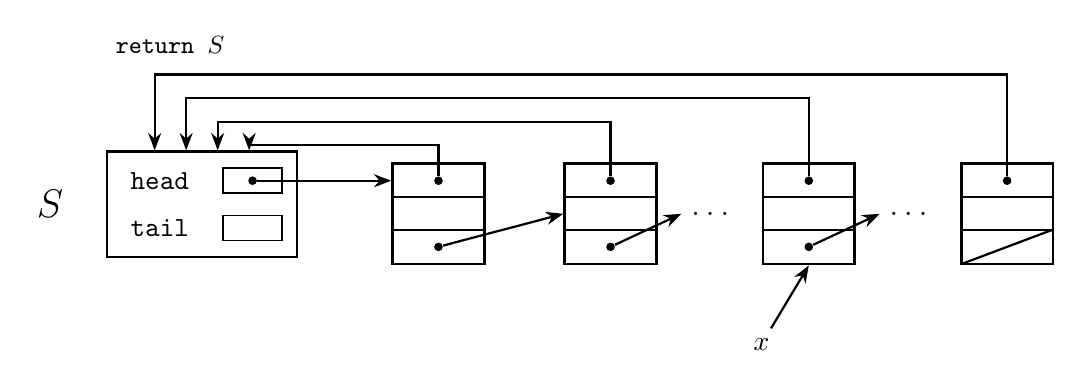
\begin{tikzpicture}[
    slot/.style={draw=black, semithick, minimum width=0.75cm, minimum height=0.32cm, inner sep=0pt},
    cell/.style={draw=black, semithick, minimum width=1.15cm, minimum height=0.42cm, font=\small},
    arr/.style={-{Stealth[length=2.2mm]}, thick},
    ptr/.style={circle, fill=black, inner sep=1.1pt}
]
    % --- 1. Oggetto Insieme S (a sinistra) ---
    \node[font=\bfseries\Large] (s_lbl) at (-0.9, 0) {$S$};

    \node[anchor=west] (head_lbl) at (0, 0.3) {\texttt{head}};
    \node[slot, right=3mm of head_lbl] (head_slot) {};

    \node[anchor=west] (tail_lbl) at (0, -0.3) {\texttt{tail}};
    \node[slot, right=3mm of tail_lbl] (tail_slot) {};

    \node[draw=black, thick, fit=(head_lbl) (head_slot) (tail_lbl) (tail_slot), inner xsep=5pt, inner ysep=4pt] (boxS) {};

    % --- 2. Elementi della lista concatenata ---
    % Blocco 1 (testa)
    \node[cell, right=1.2cm of boxS.east |- head_slot] (b1_set) {};
    \node[cell, below=-\pgflinewidth of b1_set] (b1_key) {};
    \node[cell, below=-\pgflinewidth of b1_key] (b1_next) {};
    \node[draw=black, thick, fit=(b1_set) (b1_next), inner sep=0pt] (box_b1) {};

    % Blocco 2
    \node[cell, right=1.0cm of box_b1.east |- b1_set] (b2_set) {};
    \node[cell, below=-\pgflinewidth of b2_set] (b2_key) {};
    \node[cell, below=-\pgflinewidth of b2_key] (b2_next) {};
    \node[draw=black, thick, fit=(b2_set) (b2_next), inner sep=0pt] (box_b2) {};

    % Primi puntini di sospensione
    \node[right=3mm of box_b2.east |- b1_key, font=\large] (dots1) {$\dots$};

    % Blocco x
    \node[cell, right=3mm of dots1.east |- b1_set] (bx_set) {};
    \node[cell, below=-\pgflinewidth of bx_set] (bx_key) {};
    \node[cell, below=-\pgflinewidth of bx_key] (bx_next) {};
    \node[draw=black, thick, fit=(bx_set) (bx_next), inner sep=0pt] (box_bx) {};

    % Secondi puntini di sospensione
    \node[right=3mm of box_bx.east |- b1_key, font=\large] (dots2) {$\dots$};

    % Ultimo blocco (coda)
    \node[cell, right=3mm of dots2.east |- b1_set] (blast_set) {};
    \node[cell, below=-\pgflinewidth of blast_set] (blast_key) {};
    \node[cell, below=-\pgflinewidth of blast_key] (blast_next) {};
    \node[draw=black, thick, fit=(blast_set) (blast_next), inner sep=0pt] (box_blast) {};

    % Slash per puntatore NIL nell'ultimo blocco
    \draw[thick] (blast_next.south west) -- (blast_next.north east);

    % --- 3. Punti di origine dei puntatori ---
    \node[ptr] (pt_head) at (head_slot.center) {};
    \node[ptr] (pt_b1_set) at (b1_set.center) {};
    \node[ptr] (pt_b2_set) at (b2_set.center) {};
    \node[ptr] (pt_bx_set) at (bx_set.center) {};
    \node[ptr] (pt_blast_set) at (blast_set.center) {};
    \node[ptr] (pt_b1_next) at (b1_next.center) {};
    \node[ptr] (pt_b2_next) at (b2_next.center) {};
    \node[ptr] (pt_bx_next) at (bx_next.center) {};

    % --- 4. Collegamenti orizzontali (head e next) ---
    \draw[arr] (pt_head) -- (box_b1.west |- b1_set);
    \draw[arr] (pt_b1_next) to[out=15, in=195] (box_b2.west |- b2_key);
    \draw[arr] (pt_b2_next) -- (dots1.west);
    \draw[arr] (pt_bx_next) -- (dots2.west);

    % --- 5. Variabile x puntata dal basso verso il blocco x ---
    \node (x_var) at ([shift={(-0.6cm, -1.0cm)}]box_bx.south) {$x$};
    \draw[arr] (x_var) -- (box_bx.south);

    % --- 6. Puntatori di ritorno verso l'oggetto S (operazione Find-Set) ---
    \draw[arr] (pt_b1_set) -- ++(0, 0.45) -| ([xshift=6mm]boxS.north);
    \draw[arr] (pt_b2_set) -- ++(0, 0.75) -| ([xshift=2mm]boxS.north);
    \draw[arr] (pt_bx_set) -- ++(0, 1.05) -| ([xshift=-2mm]boxS.north);
    \draw[arr] (pt_blast_set) -- ++(0, 1.35) -| ([xshift=-6mm]boxS.north);

    % Etichetta "return S"
    \node[anchor=south west, font=\small\ttfamily] at ([yshift=1.1cm]boxS.north west) {return $S$};

\end{tikzpicture}
\caption{Funzionamento dell'operazione \textsc{Find-Set}($x$) in tempo $O(1)$ tramite puntatore diretto all'oggetto insieme $S$.}
\end{figure}

\newpage
\subsection{Union}
La più semplice implementazione dell'operazione Union che usa la rappresentazione degli insiemi mediante liste concatenate richiede molto più tempo rispetto all'operazione Make-Set o Find-Set.

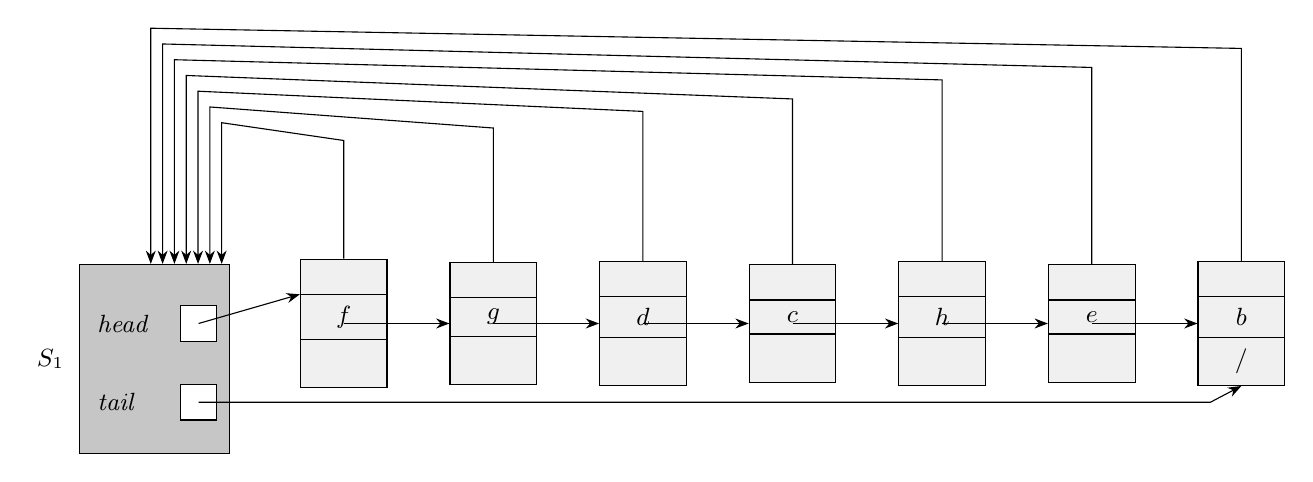
\begin{tikzpicture}[
    >=Stealth,
    font=\small,
    % Stile per i nodi della lista (3 campi verticali)
    listnode/.style={
        rectangle split,
        rectangle split parts=3,
        draw,
        fill=gray!12,
        minimum width=1.1cm,
        rectangle split part fill={gray!12, white, gray!12},
        inner sep=4pt
    },
    % Stile per l'intestazione dell'insieme
    setheader/.style={
        draw,
        fill=gray!45,
        minimum width=1.9cm,
        minimum height=2.4cm,
        inner sep=0pt
    },
    % Puntatori interni (quadratini bianchi)
    ptmbox/.style={
        draw,
        fill=white,
        minimum size=0.45cm,
        inner sep=0pt
    }
]


    % Blocco Insieme (Header)
    \node[setheader] (S) at (0, 0) {};
    \node[left=2pt of S.west] {$S_1$};

    % Testo ed elementi interni all'Header
    \node[anchor=west] at ([xshift=3pt, yshift=0.45cm]S.west) {\textit{head}};
    \node[ptmbox] (head_box) at ([xshift=-0.4cm, yshift=0.45cm]S.east) {};

    \node[anchor=west] at ([xshift=3pt, yshift=-0.55cm]S.west) {\textit{tail}};
    \node[ptmbox] (tail_box) at ([xshift=-0.4cm, yshift=-0.55cm]S.east) {};

    % Nodi della lista concatenata
    \node[listnode] (N1) at (2.4, 0.45) {\nodepart{two}$f$\nodepart{three}\phantom{/}};
    \node[listnode] (N2) at (4.3, 0.45) {\nodepart{two}$g$\nodepart{three}\phantom{/}};
    \node[listnode] (N3) at (6.2, 0.45) {\nodepart{two}$d$\nodepart{three}\phantom{/}};
    \node[listnode] (N4) at (8.1, 0.45) {\nodepart{two}$c$\nodepart{three}\phantom{/}};
    \node[listnode] (N5) at (10.0, 0.45) {\nodepart{two}$h$\nodepart{three}\phantom{/}};
    \node[listnode] (N6) at (11.9, 0.45) {\nodepart{two}$e$\nodepart{three}\phantom{/}};
    \node[listnode] (N7) at (13.8, 0.45) {\nodepart{two}$b$\nodepart{three}/};

    % Puntatore head -> primo elemento
    \draw[->] (head_box.center) -- (N1.text split west);

    % Puntatori next tra elementi consecutivi
    \foreach \i/\j in {1/2, 2/3, 3/4, 4/5, 5/6, 6/7} {
        \draw[->] (N\i.three split) -- (N\j.three split west);
    }

    % Puntatore tail -> ultimo elemento
    \draw[->] (tail_box.center) -- ++(12.85, 0) -- (N7.south);

    % Puntatori dai campi superiori dei nodi verso la testa dell'insieme S1
    % Ogni linea ha una quota orizzontale progressiva e un punto di arrivo distinto sulla testa di S
    \foreach \i/\h/\xoffset in {
        1/1.95/0.85,
        2/2.15/0.70,
        3/2.35/0.55,
        4/2.55/0.40,
        5/2.75/0.25,
        6/2.95/0.10,
        7/3.15/-0.05
    } {
        \draw[->] (N\i.north) 
            -- ++(0, \h - 0.45) 
            -- ([xshift=\xoffset cm]S.north |- 0, \h + 1.05) 
            -- ([xshift=\xoffset cm]S.north);
    }

\end{tikzpicture}



Eseguiamo la Union(x,y) aggiungendo la lista y alla fine della lista .

Il rappresentante della lista x diventa il rappresentante della lista finale. 

Purtroppo dobbiamo aggiornare il puntatore all'oggetto dell'insieme per ogni oggetto che originariamente si trovava nella lista, questo richiede un tempo lineare nella lunghezza della lista y.

Eseguiamo $n$ operazioni Make-Set, seguite da $n-1$ operazioni Union, quindi $m=2n-1$. 
Impieghiamo un tempo $\Theta(n)$ per eseguire le $n$ operazioni Make-Set. Poichè l'i-esima operazione Union aggiorna $i$ oggetti, il numero totale di oggetti aggiornati da tutte le $n-1$ operazioni Union è

{
    \Large
    \[
        \sum^{n-1}_{i=1} i = \mathbf{\Theta(n^2)}
    \]
}

\begin{center}
    \begin{algorithmic}[1]
        \Procedure{Union}{$x, y$}
            \State $S_1 \gets x.set$
            \State $S_2 \gets y.set$
            \State $S_1.tail.next \gets S_2.head$
            \State $S_1.tail \gets S_2.tail$
            \State $z \gets S_2.head$
            \While{$z \neq \text{NIL}$}
                \State $z.set \gets S_1$
                \State $z \gets z.next$
            \EndWhile
            \State \Return $S_1$
        \EndProcedure
    \end{algorithmic}
\end{center}

\newpage
\section{Euristica dell'unione pesata}
Nel caso peggiore, l'implementazione dell'operazione UNION richiede un tempo medio $\Theta(n)$ per chiamata, perchè potremmo appendere una lista più lunga a una più corta, dobbiamo aggiornare il puntatore all'oggetto dell'insieme per ogni elemento della lista più lunga.

Supponiamo invece che:
\begin{itemize}
    \item Ogni lista includa anche la sua lunghezza
    \item Appendiamo ogni volta la lista più corta a quella più lunga, risolvendo in modo arbitrario i casi di liste aventi la stessa lunghezza
\end{itemize}

Con questa \textbf{euristica dell'unione pesata}, una singola operazione UNION può ancora impiegare $\Omega(n)$ se entrambe le liste hanno $\Omega(n)$ elementi.

Tuttavia, una sequenza di $m$ operazioni Make-Set,Union e Find-Setn $n$ delle quali sono perazioni Make-Set, impiega un tempo $O(m+n\log(n))$

\subsection{Teorema}
Utilizzando la rappresentazione degli insiemi disgiunti tramite liste concatenate e l'euristica dell'unione pesata, una sequenza di $m$ operazioni Make-Set, Union e Find-Set, $n$ delle quali sono operazioni Make-Set, impiega un tempo $O(m+n\log(n))$

\subsection{Dimostrazione}
Sia $x$ un qualunque oggetto (ce ne sono $n$) calcoliamo il massimo numero di volte che x.set viene aggiornato. Ogni volta che x.set viene aggiornato x si deve trovare nella lista più corta

\begin{table}[htbp]
\centering
\renewcommand{\arraystretch}{1.5}
    \begin{tabular}{lll}
    $1^{\text{a}}$ volta che \texttt{x.set} viene aggiornato & l'insieme risultante ha almeno & $2$ elementi \\
    $2^{\text{a}}$ volta che \texttt{x.set} viene aggiornato  & l'insieme risultante ha almeno & $2^2$ elementi \\
    \hspace{2.3em} $\vdots$ & & \\
    $i\text{-ma}$ volta che \texttt{x.set} viene aggiornato & l'insieme risultante ha almeno & $2^i$ elementi
    \end{tabular}
\end{table}

Quindi x.set è aggiornato al massimo $\log(n)$ volte. Questo perchè se fosse aggiornato più di $\log(n)$ volte l'insieme risultante avrebbe \textbf{almeno}

$$
    2^{\log(n)} > n \text{ elementi} \implies \text{Impossibile}
$$

Siccome ci sono $n$ oggetti il costo è $\mathbf{O(n+n\log(n))}$

\subsection{Algoritmo}
\begin{algorithmic}[1]
\Procedure{Union}{$x, y$}
    \State $S_1 \gets x.\textit{set}$
    \State $S_2 \gets y.\textit{set}$
    \If{$S_1 == S_2$}
        \State \Return $S_1$
    \EndIf
    \If{$S_1.\textit{length} \ge S_2.\textit{length}$}
        \State $S_1.\textit{tail}.\textit{next} \gets S_2.\textit{head}$
        \State $S_1.\textit{tail} \gets S_2.\textit{tail}$
        \State $z \gets S_2.\textit{head}$
        \While{$z \neq \text{NIL}$}
            \State $z.\textit{set} \gets S_1$
            \State $z \gets z.\textit{next}$
        \EndWhile
        \State $S_1.\textit{length} \gets S_1.\textit{length} + S_2.\textit{length}$
        \State \Return $S_1$
    \Else
        \State $S_2.\textit{tail}.\textit{next} \gets S_1.\textit{head}$
        \State $S_2.\textit{tail} \gets S_1.\textit{tail}$
        \State $z \gets S_1.\textit{head}$
        \While{$z \neq \text{NIL}$}
            \State $z.\textit{set} \gets S_2$
            \State $z \gets z.\textit{next}$
        \EndWhile
        \State $S_2.\textit{length} \gets S_2.\textit{length} + S_1.\textit{length}$
        \State \Return $S_2$
    \EndIf
\EndProcedure
\end{algorithmic}